\section{Key-Vector Norms Are Not Fixed}
\label{app:key-norms}

\paragraph{Setup.}
We run \texttt{Qwen2.5-7B-Instruct} (\texttt{fp16}, eager attention) on a
short technical prompt and decode $128$ greedy tokens, hooking every
attention layer to record the post-RoPE key vector $k_{\ell,h,t}$ for each
layer $\ell$, KV-head $h$, and token position $t$. We then compute the L2
norm $\|k_{\ell,h,t}\|_2$ and study how it varies across the three axes.
Aggregated over all $(L,H,T)=(28,4,193)$ entries the norm spans
$[0.37,\,923]$ with mean $40.0$ and standard deviation $100.1$; the
$\max/\min$ ratio is $\approx 2.5\times 10^{3}$, i.e.\ keys are far from
unit-normalised. Marginalising one axis at a time, the per-layer mean still
varies by $17\times$, the per-head mean by $2.5\times$, and the per-position
mean by $1.4\times$, so the variation is not noise but structured along each
axis. Figure~\ref{fig:keynorm-box} shows the within-layer distribution and
makes the depth dependence explicit; Figure~\ref{fig:keynorm-pos} shows the
mean and $\pm 1\sigma$ envelope at each position, revealing systematic
spikes at the BOS / system-header tokens and around the
prompt$\rightarrow$decode boundary.

\paragraph{Implication for sparse attention.}
Attention scores $s_{t,j} = q_t^\top k_j / \sqrt{d}$ scale linearly with
$\|k_j\|$, so the norm is a real component of relevance: a key with large
$\|k\|$ contributes more mass under any query whose direction is not
orthogonal to it. Index structures that normalise keys away (cosine
similarity, MIPS reductions to angular search) therefore discard a signal
the model itself produced; in contrast, half-space range searching on the
raw key vectors preserves the magnitude and treats the score threshold $T$
in the units the attention layer uses. This is one of the reasons we model
sparse attention as range searching rather than as nearest-neighbour or
cosine retrieval.

\begin{figure}[h]
  \centering
  % 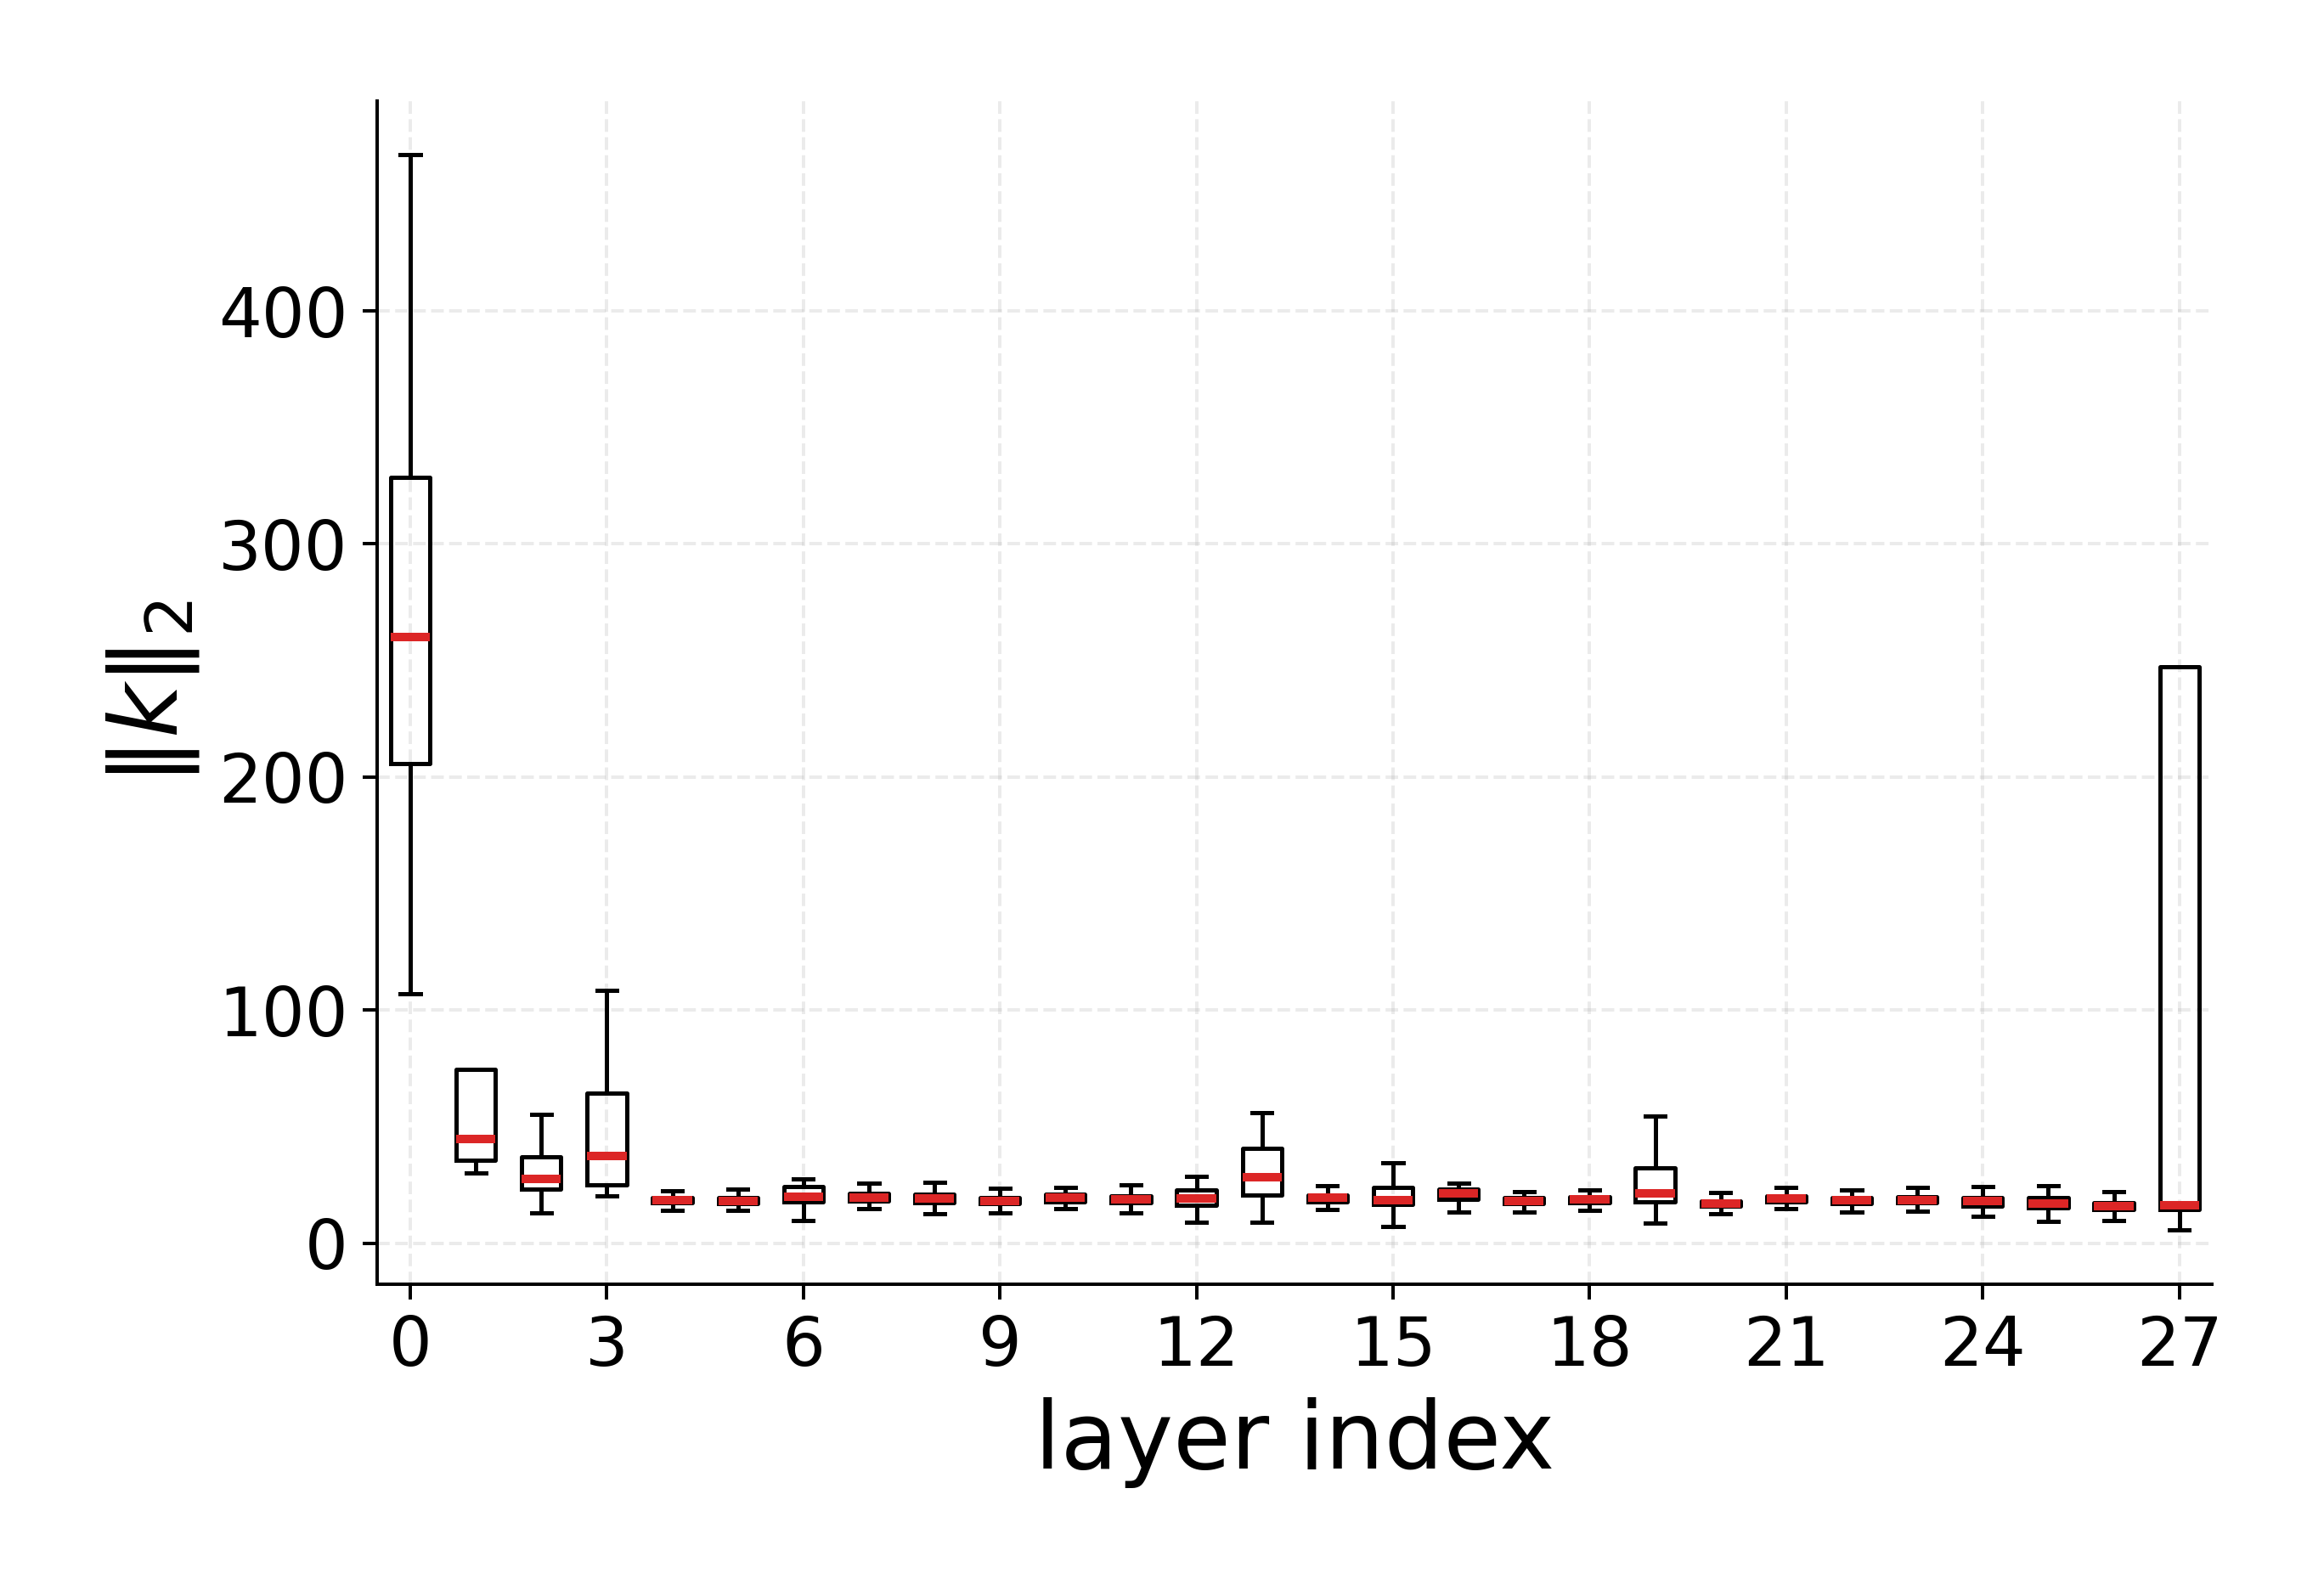
\includegraphics[width=0.7\linewidth]{figs/norm_per_layer_box.png}
  \caption{Per-layer distribution of key-vector L2 norms across all KV-heads
  and token positions in a $128$-token Qwen2.5-7B trace. The within-layer
  spread is wide and the median grows substantially with depth, so a single
  global norm assumption is not justified.}
  \label{fig:keynorm-box}
\end{figure}

\begin{figure}[h]
  \centering
  % 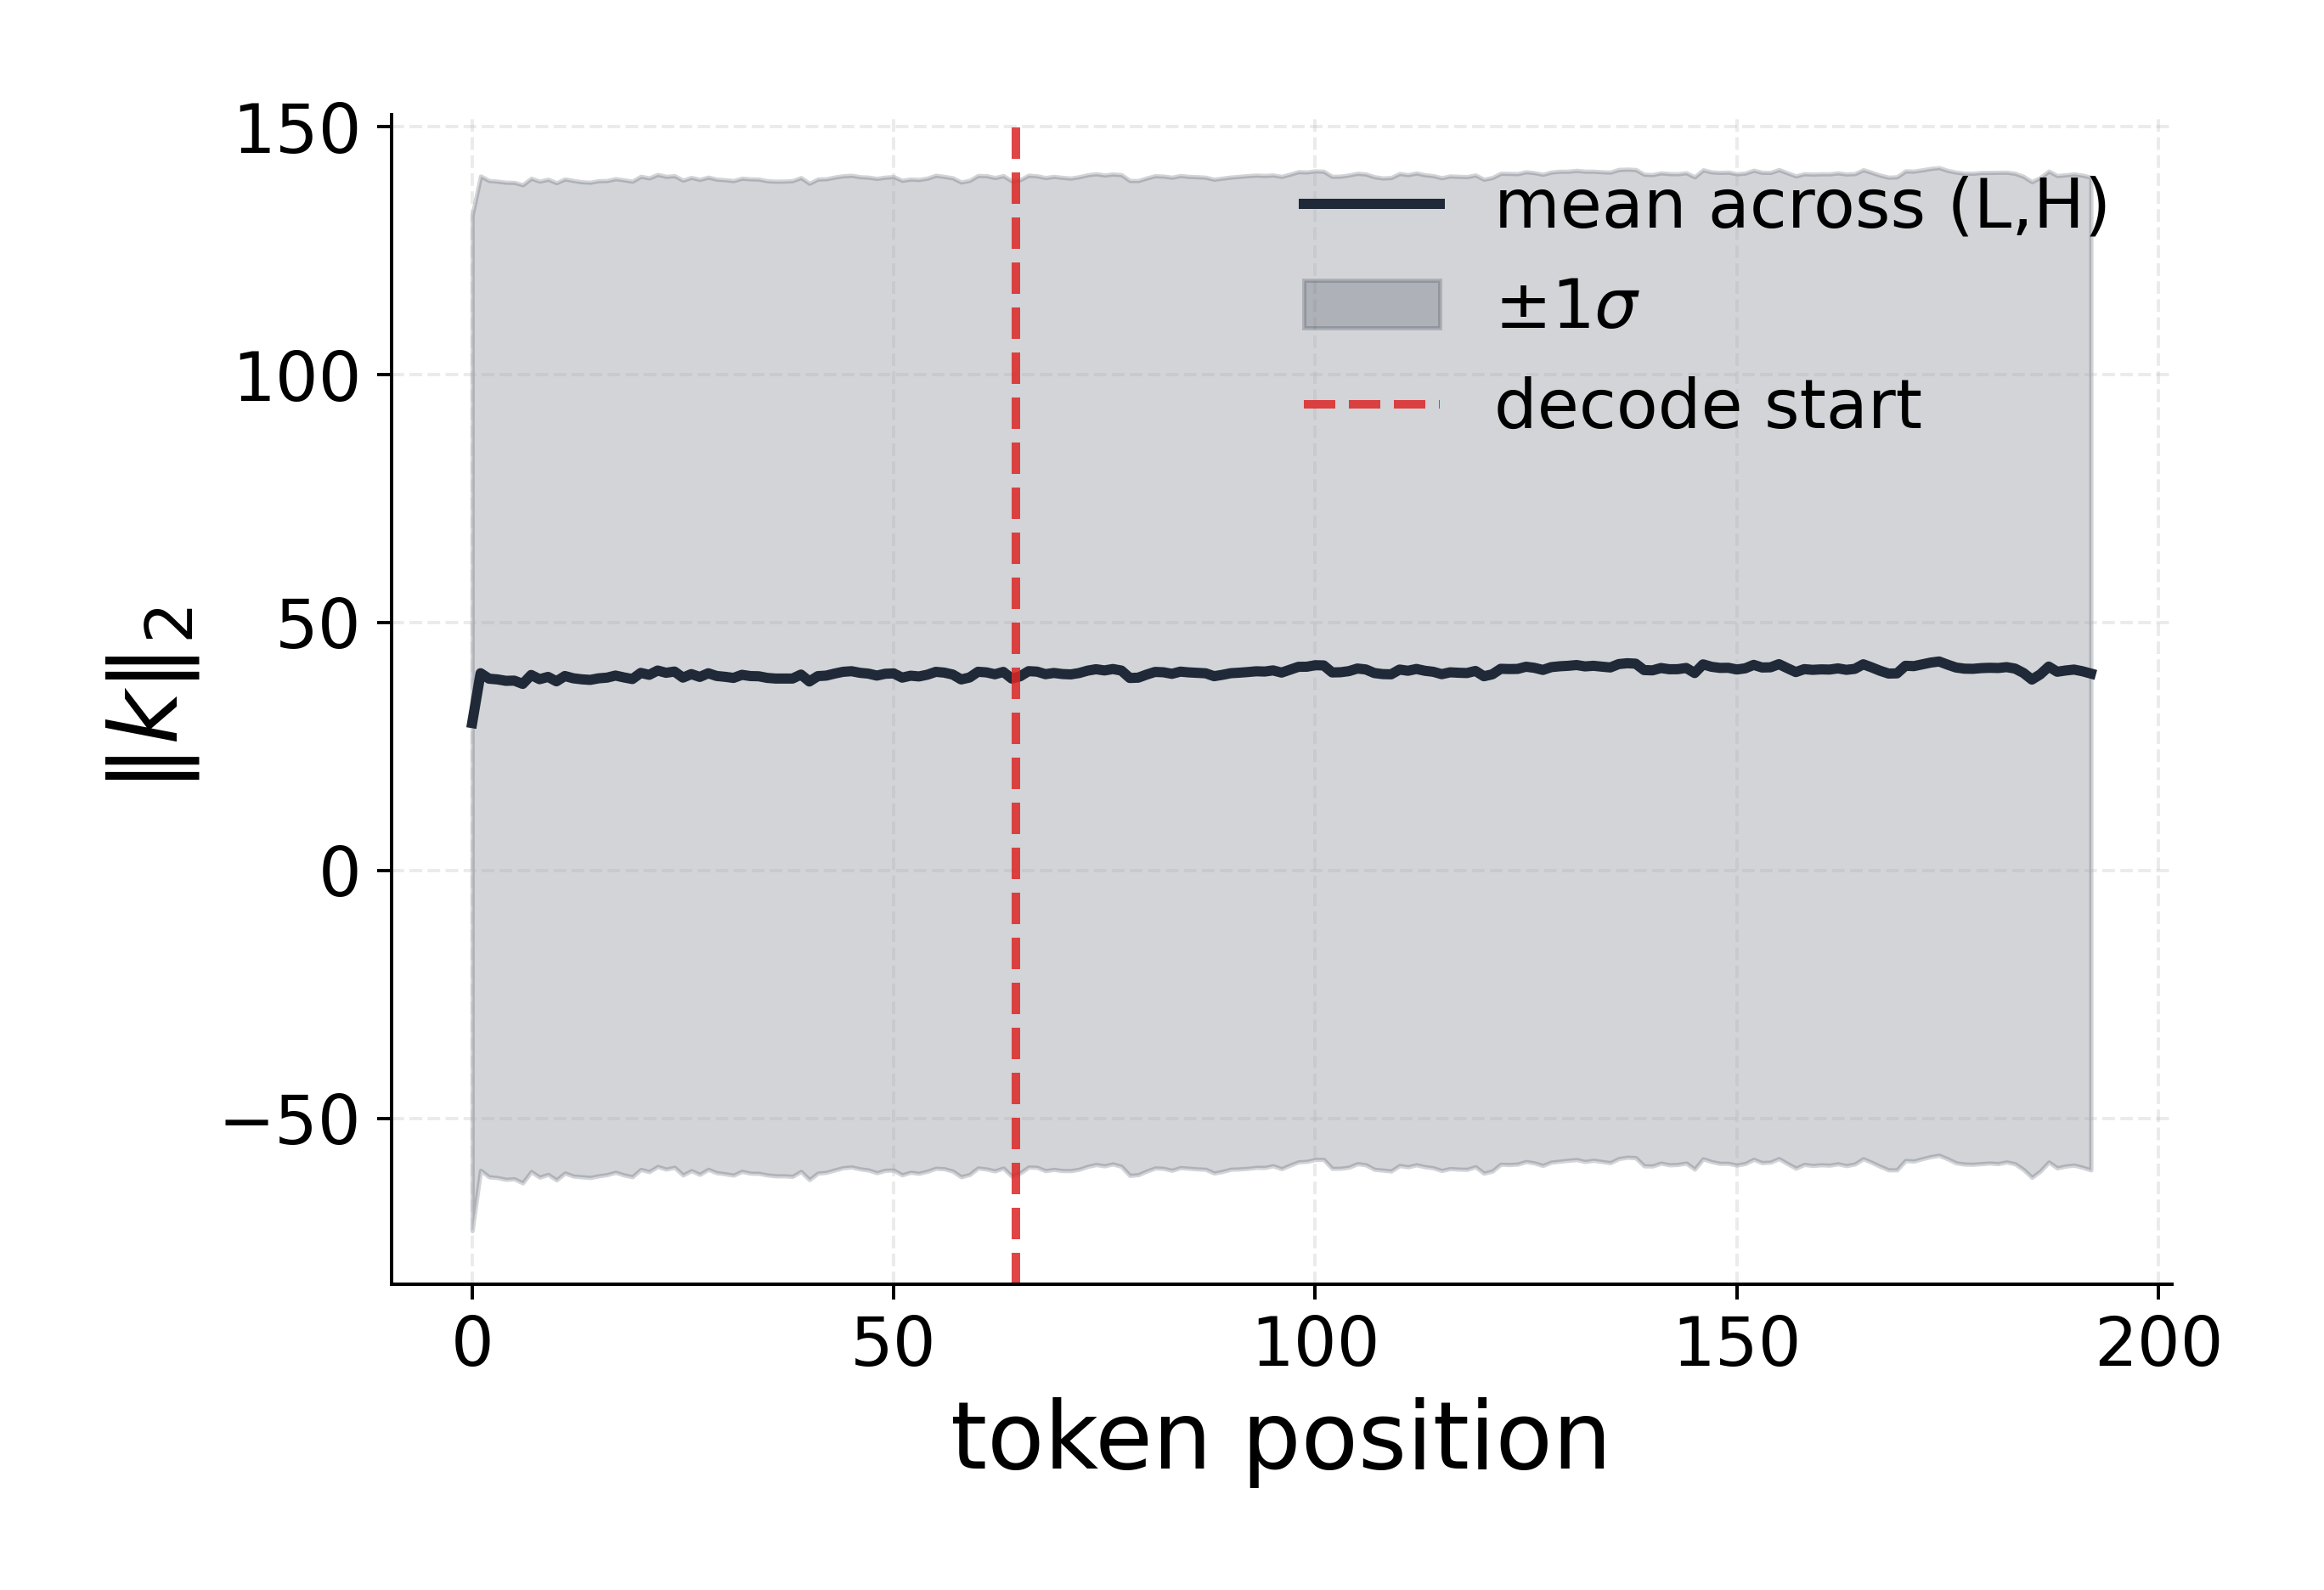
\includegraphics[width=0.7\linewidth]{figs/norm_position_meanstd.png}
  \caption{Mean key-norm at each token position (averaged across all
  $L\times H$ heads) with a $\pm 1\sigma$ envelope. The dashed line marks
  the prompt$\rightarrow$decode boundary. Norms peak at the first few
  positions (BOS / system header) and exhibit position-dependent drift
  rather than a constant value.}
  \label{fig:keynorm-pos}
\end{figure}
